\section{Introduction}\label{paperA:sec:introduction}

In this paper, we focus on the application of image recognition models implemented into assistive technologies for people with visual impairments. Such technologies already exist in the form of mobile applications, e.g.~Microsoft's Seeing AI \citeA{seeingAImicrosoft} and Aipoly Vision \citeA{aipolyvision}, and as wearable artificial vision devices, e.g.~Orcam MyEye \citeA{orcam} and the Sound of Vision system introduced in \citeA{paperA:caraiman2017soundofvision}. These products have the ability to support people with visual impairments in many different situations, such as reading text documents, describing the user's environment and recognizing people the user may know. 

\begin{figure}[t]
	\centering
    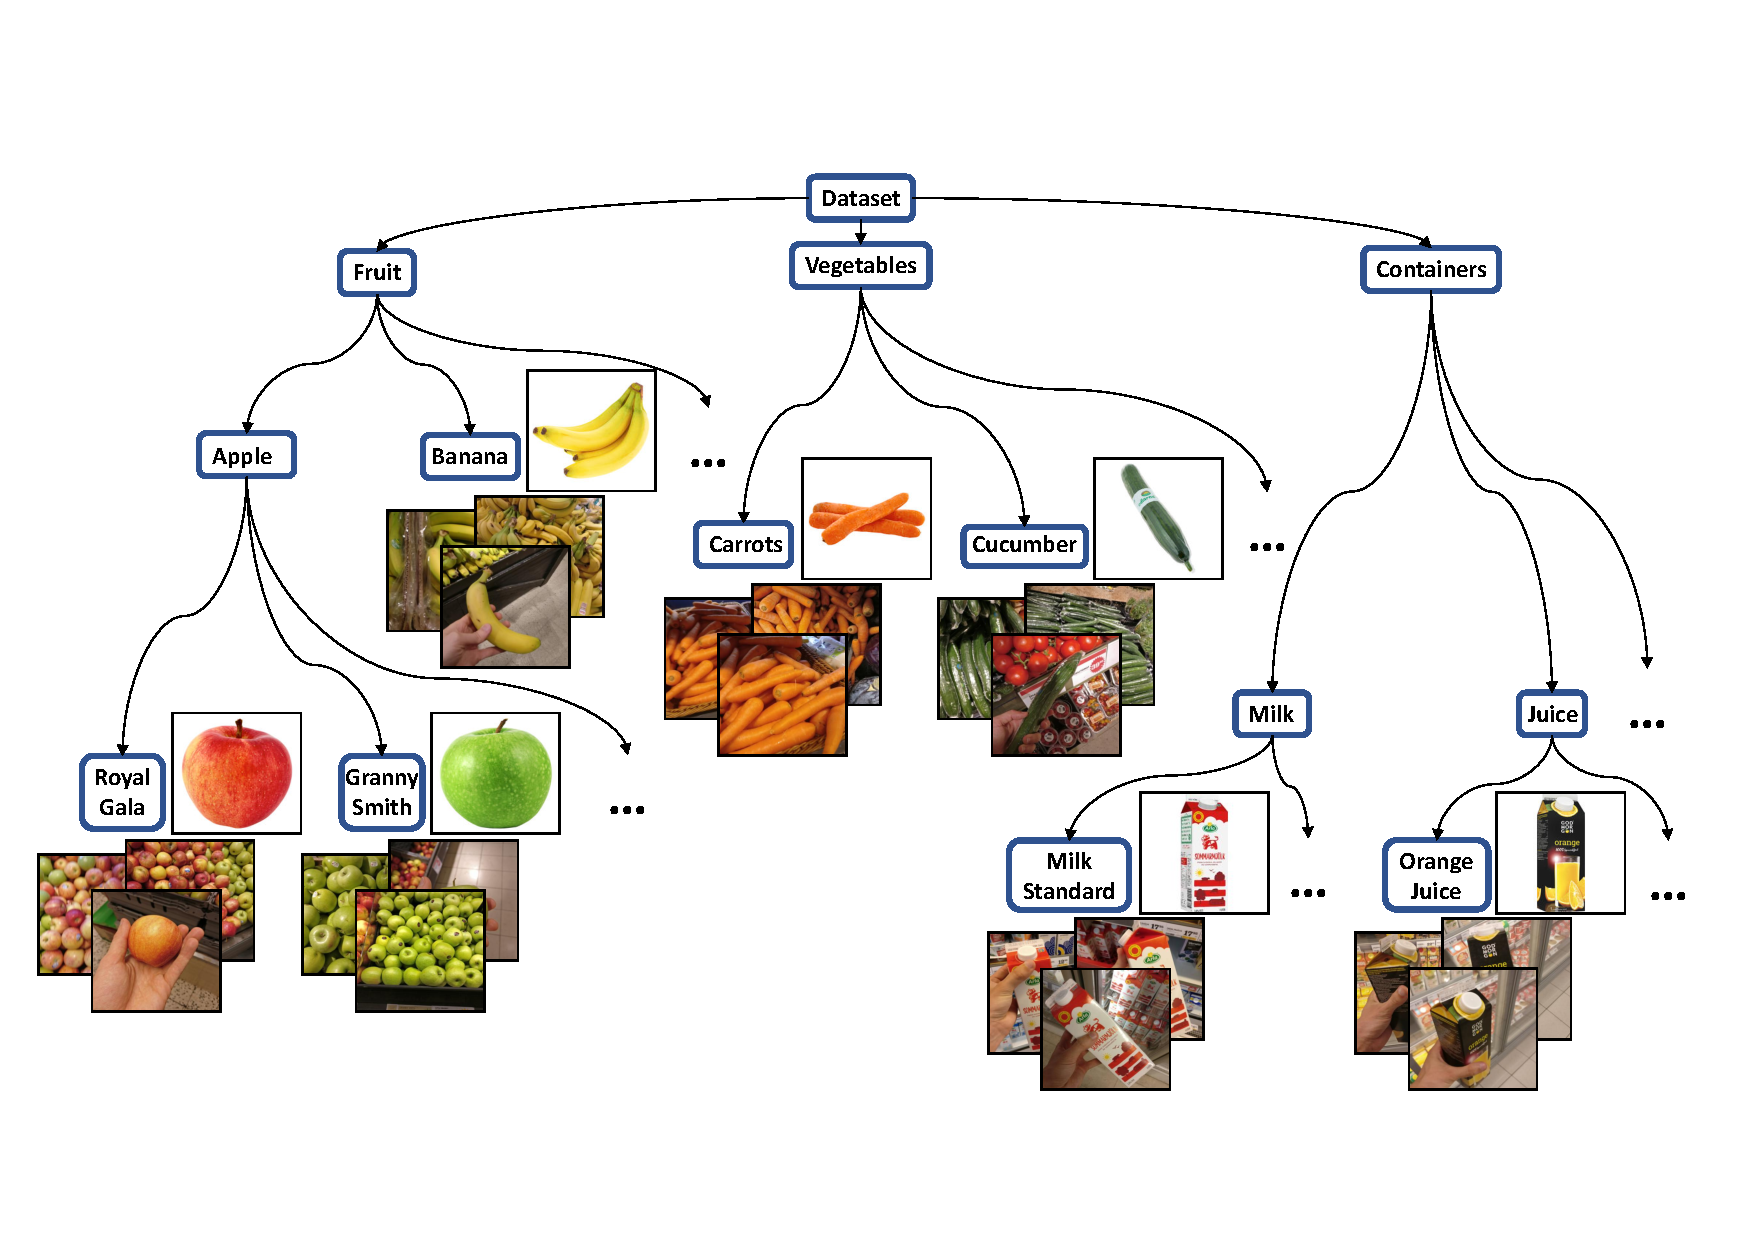
\includegraphics[width=0.9\textwidth]{PaperA/figures/intro.pdf}
    \vspace{-2mm}
    \caption{The primary contribution of this paper is a dataset of grocery items, for the purpose of training a visual recognition system to aid visually impaired people. The dataset is organized according to a hierarchical class structure, as illustrated above. A novel aspect of the dataset is that each class, apart from the semantic label, also has a visual label in the form of an iconic image.}
    \label{fig:examples} 
    \vspace{-3mm}
\end{figure}

We here address a complementary scenario not handled by current systems on the market: visual support when shopping for grocery items considering a large range of eatable objects, including fruits, vegetables, milk, and juices. 
In the case of fruits and vegetables, these are usually stacked in large bins in grocery stores as shown in Figure \ref{fig:dataset-figure}(a-f). A common problem in grocery stores is that similar items are often stacked next to each other; therefore, items are often misplaced into neighboring bins. Figure \ref{subfig:real-image-a} shows a mix of red and green apples, where it might be difficult for the system to determine which kind of apple is the actual target.
Humans can distinguish between groceries without vision to some degree, e.g.~by touching and smelling them, but it requires prior knowledge about texture and fragrance of food items.

Moreover, in addition to raw grocery items, there are also items that can only be differentiated with the help of visual information, e.g. milk, juice, and yogurt cartons, see Figure \ref{fig:dataset-figure}(g-i). Such items usually have barcodes, that are readable using the existing assistive devices described above. However, the barcodes are not easily located by visually impaired persons. Thus, an assistive vision device that fully relies on natural image understanding would be of significant added value for a visually impaired person shopping in a grocery store.

Image recognition models used for this task typically require training images collected in similar environments. However, current benchmark datasets, such as ImageNet \citeA{paperA:deng2009imagenet} and CIFAR-100 \citeA{paperA:Krizhevsky2009cifar100}, do contain images of fruits and vegetables, but are not suitable for this type of assistive application, 
since the target objects are commonly not presented in this type of natural environments, with occlusion and cluttered backgrounds. To address this issue, we present a novel dataset containing natural images of various raw grocery items and refrigerated products, e.g. milk, juice, and yogurt, taken in grocery stores. As part of our dataset, we collect images taken with single and multiple target objects, from various perspectives, and with noisy backgrounds.

In computer vision, previous studies have shown that model performance can be improved by extending the model to utilize other data sources, e.g. text, audio, in various machine learning tasks \citeA{paperA:frome2013DeVISE, paperA:Gebru2017FineGrainedCD, paperA:karpathy2015deepvisualsemantic, paperA:ngiam2011multimodal}. Descriptions of images are rather common to computer vision datasets, e.g. Flickr30k \citeA{paperA:plummer2015flickr30k}, whereas the datasets in \citeA{paperA:Gebru2017FineGrainedCD, paperA:Lin2014MicrosoftCoco} includes both descriptions and a reference image with clean background to some objects. Therefore, in addition to the natural images, we have collected iconic images with a single object centered in the image (see Figure \ref{fig:clean-image-figure}) and a corresponding product description to each grocery item. In this work, we also demonstrate how we can benefit from using additional information about the natural images by applying the multi-view generative model.

To summarize, the contribution of this paper is a dataset of natural images of raw and refrigerated grocery items, which could be used for evaluating and training image recognition systems to assist visually impaired people in a grocery store. 
The dataset labels have a hierarchical structure with both coarse- and fine-grained classes (see Figure \ref{fig:examples}). Moreover, 
each class also has an iconic image and a product description, which makes the dataset applicable to multimodal learning models. The dataset is described in Section \ref{sec:our-dataset}. 

We provide multiple benchmark results using various deep neural networks, such as Alexnet \citeA{paperA:krizhevsky2012imagenet}, VGG \citeA{paperA:simonyan2014verydeep}, DenseNet \citeA{paperA:huang2017densely}, as well as deep generative models, such as VAE \citeA{paperA:kingma2014autoencoding}. 
Furthermore, we adapt a multi-view VAE model to make use of the iconic images for each class (Section \ref{sec:classification-methods}), and show that it improves the classification accuracy given the same model setting (Section \ref{sec:experimental-results}). Last, we discuss possible future directions for fully using the additional information provided with the dataset and adopt more advanced machine learning methods, such as visual-semantic embeddings, to learn efficient representations of the images. 